\subsection{Project Charter}
The project charter shall be a key document for our project. This document defines the objectives, scope and structure for the design and development of the Smart Cart. The document will also show the schedule for sprints and establish the roles and responbilities for each team member. 

\subsection{Product Backlog}
The prodcut backlog will establish the initial requirements for the Smart Cart. The product backlog will be updated to reflect any requirements changes. All team members are responsible for checking the backlog to ensure that they are aware of the changes. All changes wil be documented and explained in this document.

\subsection{Sprint Planning}
All members of the team are required to attend to every sprint-planning meeting. The meetings will focus on completing tasks that will further progress the project. Documentations will be updated if necessary during sprint-plannings to keep everyone updated. The team will also define the sprint backlog and set the schedule for the sprint. Each sprint will be between 2 to 4 weeks.

\subsubsection{Sprint Goal}
The sprint goal is a descripion of what the team will be working towards for that sprint. This enables all team members to work towards the same goal. As the project progresses, the sprint goal will change.

\subsubsection{Sprint Backlog}
The sprint backlog is a list of tasks defined by the Scrum Master during a sprint team meeting. The tasks are split and assigned to each team member based on their strengths. This ensures that there will be progress towards the goal of each sprint. Each team member will then track the amount of hours they spent working on their tasks. New items will be added to the backlog for future sprints.

\subsubsection{Task Breakdown}
In order to complete certain tasks of the sprint backlog, the tasks will be broken down into small subtasks. Splitting the work load will ensure that each team member will complete their assigned work to the best of their abilities. Each individual is also responsible for researching and getting assistance if needed. The team will meet semi-weekly to ensure that all members are on track towards the sprint goal.

\subsection{Sprint Burndown Charts}
During each sprint, the burndown chart will change as the project progresses. The spreadsheet will have a list of tasks the estimated amount of time the team should spend on each task and the actual amount of time spend. In order to keep track of the sprint goal progress, the sprint burndown chart will be uploaded to the Google Drive folder shared by the team. This will ensure that all team members can track their progress and stay on track towards the sprint goal. An example of a sprint burndown chart is shown in Figure 1.

\begin{figure}[h!]
    \centering
    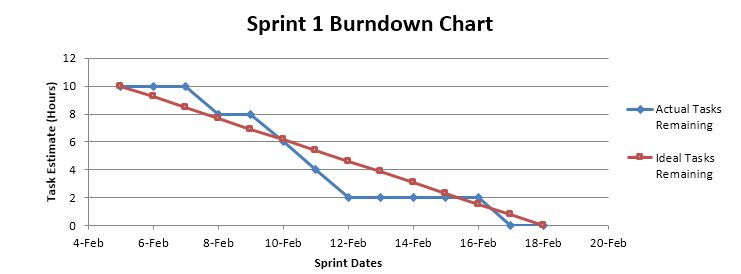
\includegraphics[width=0.80\textwidth]{images/chart}
    \caption{Sprint 1 Burndown Chart}
\end{figure}

\subsection{Sprint Retrospective}
During the sprint retrospective, the Scrum Master will debrief the team on the previous sprint session. The discussion will include improvements that could be made and other issues that need to be addressed if neccessary. This will help ensure that future sprints will be more productive and successful.

\subsection{Individual Status Reports}
Throughout the project, each team member is required to complete an individual status report. Each individual team member will record the tasks they have completed or are currently working on, the number of hours spent on each tasks and their future plans for the next sprint. If any unexpected tasks occurs, it will also be recorded.

\subsection{Engineering Notebooks}
Each team member is required to keep an Engineering notebook for the project. The notebook will contain details of each group meeting and any important ideas a team member finds. Any related work that is done outside of group time will also be recorded in the notebook. These notebooks are crucial for each team member since it is a legal document that tracks the teams' progress. 

\subsection{Closeout Materials}
\subsubsection{System Prototype}
During the development cycle, the team will develop a functioning prototype of the Smart Cart. As the project progresses, modifications to the prototype will be performed. All testing related to the project will be performed on the prototype. 

\subsubsection{Project Poster}
The project poster will include details of our project such as our vision, mission, and success criteria. This poster will be useful for presenting our project at UTA's outreach program.

\subsubsection{Demo Video}
The team will make a video to demonstrate the project. The video will explain how the cart will operate and the Smart Cart will demonstrate its intended functions.

\subsubsection{Source Code}
The source code will be stored on GitHub so the team can work on the software at their own pace. At this time, the project will be programmed in C++.

\subsubsection{Source Code Documentation}
The team will keep detailed documentation in the source code for the project. The purpose of the source code documentation is to explain the functions. This will allow future teams to easily understand the source code and make modification to the product.

\subsubsection{Hardware Schematics}
This project involves interfacing multiple hardware devices (Intel RealSense, Omni Wheels, Stepper motors), a camera module, electronic components and a power supply. The schematic diagram of the product will be the vital documentation that the team will provide.

\subsubsection{CAD files}
The team currently does not anticipate to have any CAD files. If any 3D printing is to be done later on, we will use the opensource GrabCad to find relevant files.

\subsubsection{User Manual}
The team will provide a user manual to explain how the Smart Cart will work. It will include details on how to power on, operate and power off the cart. It will also contain safety concerns and precautions.